\documentclass{icorsdssv2024}
\graphicspath{{../figures/}{../code/notebooks/pic}}
\usepackage[outline]{contour}
\usepackage{subcaption}
\usepackage{float}
%\usepackage[export]{adjustbox}[2011/08/13]
%\captionsetup[subfigure]{labelformat=empty}
%\usepackage{lipsum}

\begin{document}


%%%%%%%%%%%%%%%%%%%%%%%%%%%%%%%%%%%%%%%%%%%%%%%%%%%%%%%%%%%%%%%%%%%
%          BELOW THIS LINE YOU CAN MODIFY WITH YOUR DATA          %
%%%%%%%%%%%%%%%%%%%%%%%%%%%%%%%%%%%%%%%%%%%%%%%%%%%%%%%%%%%%%%%%%%%

% Title and running title (short title) to be used as header
\mytitle{Influence of hyperparameters on online aggregation with countable experts}
\mytitlerunning{Online experts aggregation}

% Authors and running list of authors to be used as header
% Author names must be included as: "N. Surname"
% Author names for running titles must be specified as:
% For one author: N. Surname
% For two authors: N1. Surname1 and N2. Surname2
% For more than two authors: N1. Surname \emph{et al.}
% Use \underline for the presenter.

\myauthor{S.\,M.~Kunin-Bogoiavlenskii$^{1\ast}$, A.\,V.~Zukhba$^1$, R.\,D.~Zukhba$^1$}
\myauthorrunning{S.\,M.~Kunin-Bogoiavlenskii \emph{et al.}}

% Full address for correspondence and e-mail of all authors
\myaddress{$^1$Moscow Insitute of Physics and Technology
\\ kunin-bogoiavlenskii.sm@phystech.edu; a\_\_l@mail.ru; zukhba.rd@phystech.edu \\ $^{*}$Presenting author}
\abstract{
Aggregating forecasts from multiple experts is a valuable method to improve prediction accuracy.
    Our work examines the influence of hyperparameters on the accuracy of the aggregation algorithm for a countable number of experts.
    We implement a time series generator with specified properties and an aggregating forecasting model. 
    We conduct a series of experiments with various hyperparameters of the algorithm 
%    (including initialization weights, mixing scheme, train window). 
    The experiments confirm that these hyperparameters have a significant influence on the algorithm's performance. }
% Keywords (at most 5)
\mykeywords{online learning; aggregating algorithm; prediction with experts’ advice; Fixed Share, Mixing Past Posteriors (MPP)}
\myudc{519.246 + 519.837}
\mymaketitle

Our work focuses on the problem of online time series forecasting using expert advice, particularly when dealing with a countable number of experts. 
This means that the pool of potential experts is not fixed beforehand, but rather new experts can be introduced dynamically over time.
Inspired by the algorithm developed in \cite{article}, which handles online prediction with countable experts, we investigate the role of hyperparameter optimization in achieving optimal performance. 
Our approach makes no assumptions about the underlying nature of the data, allowing it to handle deterministic, stochastic, or other types of time series.

The standard online learning framework for prediction with expert advice involves a master algorithm aggregating predictions from a set of expert models. 
At each time step, the master algorithm combines expert predictions, makes its own prediction, and then receives feedback in the form of a loss function. 
The goal is to minimize the difference between the master's cumulative loss and the best expert's cumulative loss, a metric known as regret.
Traditional algorithms like Fixed Share \cite{article98} and Mixing Past Posteriors (MPP) \cite{article02} assume a fixed set of experts. 
However, in many real-world scenarios, the set of experts can expand dynamically. 
This necessitates algorithms capable of handling countable expert sets, such as the GMPP algorithm proposed in \cite{article}, where a new expert is introduced at each time step.

We explore how key hyperparameters affect the GMPP algorithm's performance. 
We use a synthetic time series generator with specific properties to conduct an experimental study, which helps us control the underlying data dynamics and evaluate the impact of different hyperparameter configurations.

\begin{figure}[H]
\makebox[\linewidth][c]{
\begin{subfigure}[b]{.6\textwidth}
\centering
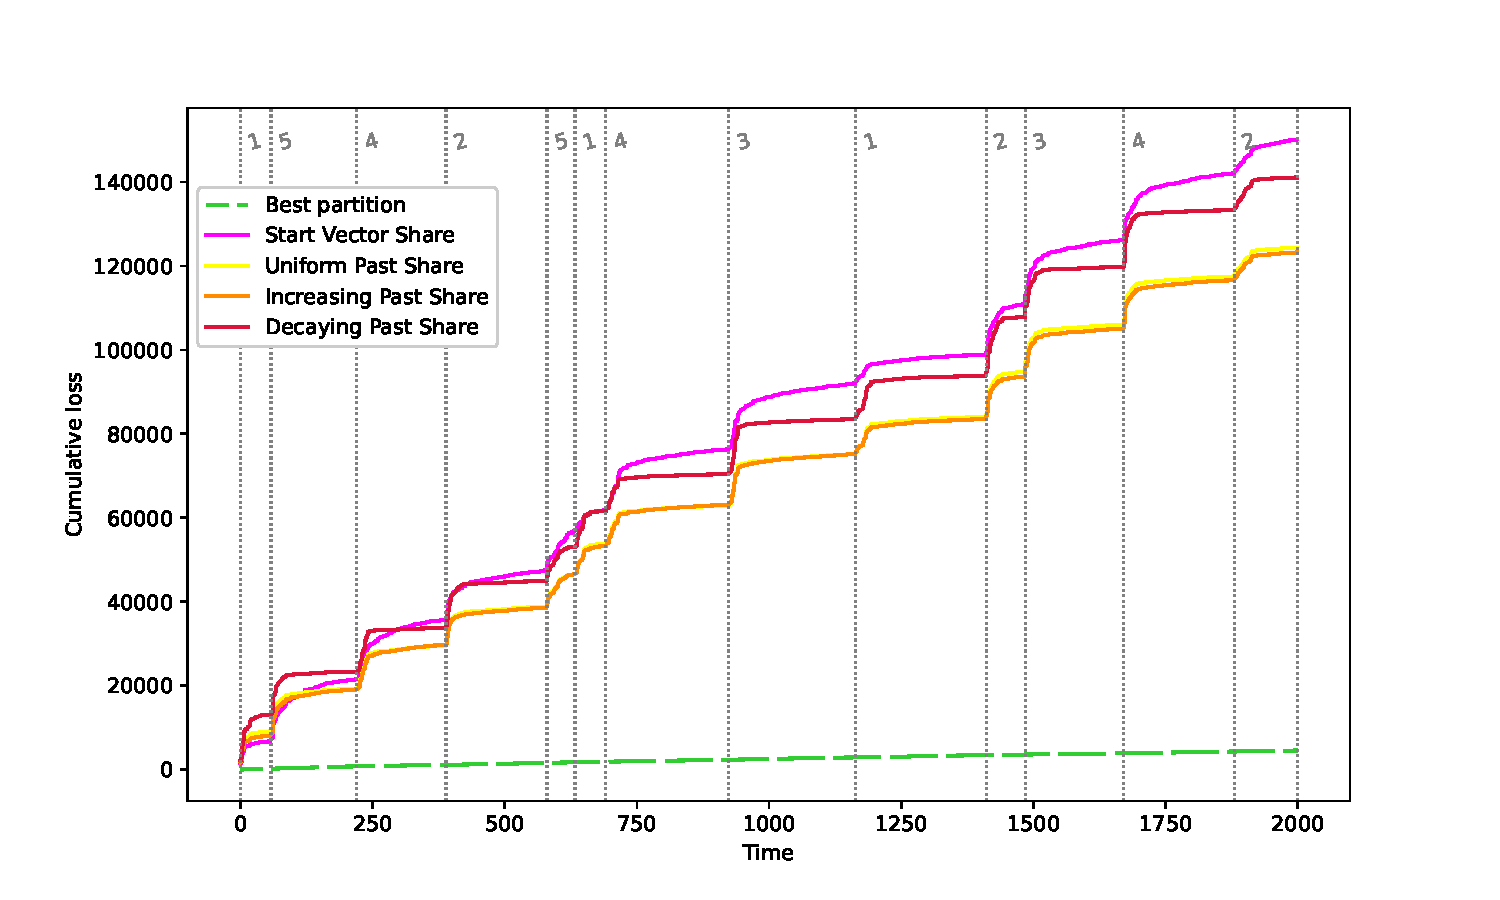
\includegraphics[width=.95\textwidth]{diff_mt}
\caption{Total losses for different mixing schemes}
\label{fig:mt}
\end{subfigure}%
\begin{subfigure}[b]{.6\textwidth}
\centering
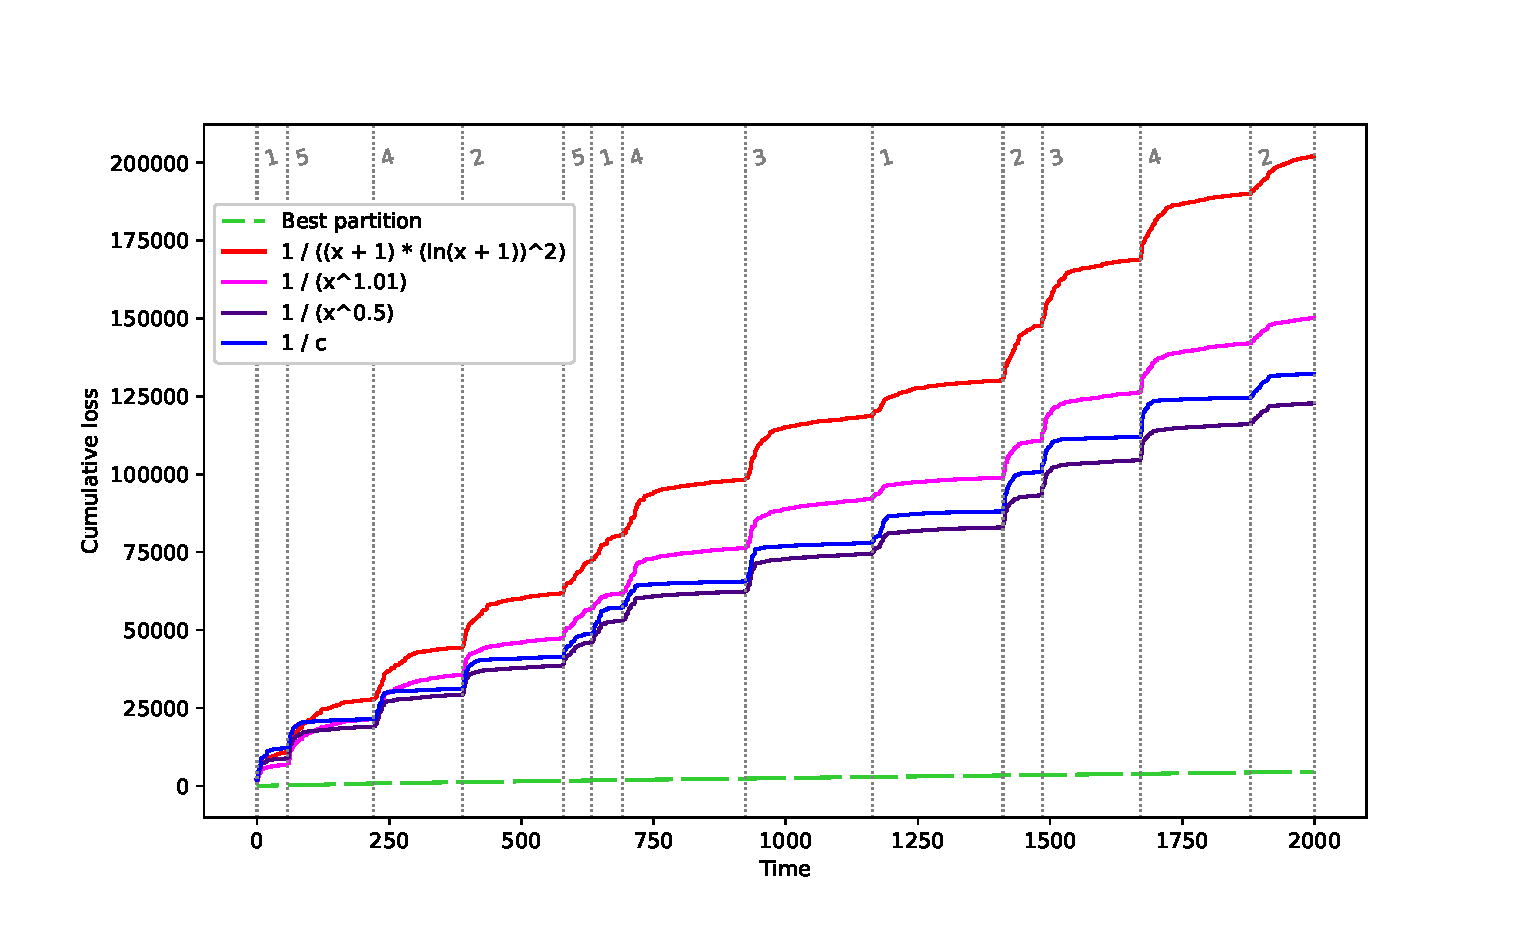
\includegraphics[width=.95\textwidth]{diff_wf}
\caption{Total losses for different weight functions}
\label{fig:wf}
\end{subfigure}
}
\caption{Total losses of the best partition and the master algorithms }
\end{figure}

Figures \ref{fig:mt} and \ref{fig:wf} illustrate the algorithm's performance under different hyperparameter settings.  
As the metric of our experiments, we use regret - the difference between the master algorithm's cumulative loss and the cumulative loss of the best partition. 
%This best partition is determined retrospectively, by dividing the time series into segments and assigning to each segment the expert that achieves the lowest cumulative loss within that segment. 
Figure \ref{fig:mt} compares the cumulative loss of the master algorithm using different mixing update schemes, including "Start Vector Share", the default scheme in \cite{article}. 
Figure \ref{fig:wf} depicts the cumulative loss using different weight initialization functions, including the default function $1 / ((x + 1)\ln^2(x + 1))$. 
These examples demonstrate the significant influence of mixing schemes and weight functions on the GMPP algorithm's performance.

Our findings highlight the importance of  considering hyperparameter choices when deploying the GMPP algorithm for online time series forecasting with countable experts. Different mixing schemes and weight initialization functions can significantly impact the algorithm's cumulative loss. In our paper we explore the effects of other hyperparameters, such as the training window size, noise variance and weights update parameters.
A comprehensive understanding of these factors may guide the development of more effective and robust online aggregation strategies for countable expert sets.


\bibliographystyle{unsrt}
\bibliography{ref}

\end{document}
